\documentclass[10pt,twocolumn,letterpaper]{article}

\usepackage{cvpr}
\usepackage{times}
\usepackage{epsfig}
\usepackage{graphicx}
\usepackage{amsmath}
\usepackage{amssymb}
\usepackage{float}
\usepackage[super]{nth}
\setlength{\textfloatsep}{5pt}

% Include other packages here, before hyperref.

% If you comment hyperref and then uncomment it, you should delete
% egpaper.aux before re-running latex.  (Or just hit 'q' on the first latex
% run, let it finish, and you should be clear).
\usepackage[breaklinks=true,bookmarks=false]{hyperref}

\cvprfinalcopy % *** Uncomment this line for the final submission

\def\cvprPaperID{****} % *** Enter the CVPR Paper ID here
\def\httilde{\mbox{\tt\raisebox{-.5ex}{\symbol{126}}}}

% Pages are numbered in submission mode, and unnumbered in camera-ready
%\ifcvprfinal\pagestyle{empty}\fi
\setcounter{page}{1}
\begin{document}

%%%%%%%%% TITLE
\title{Pattern Recognition Coursework 1}

\author{Jakub Mateusz Szypicyn\\
CID: 00846006\\
EEE4\\
{\tt\small jms13@ic.ac.uk}
% For a paper whose authors are all at the same institution,
% omit the following lines up until the closing ``}''.
% Additional authors and addresses can be added with ``\and'',
% just like the second author.
% To save space, use either the email address or home page, not both
\and
Jacobus Jukka Hertzog\\
CID: \\
EEE4\\
{\tt\small jjh13@ic.ac.uk}
}

\maketitle
%\thispagestyle{empty}

%%%%%%%%% ABSTRACT
\begin{abstract}

Line1\\

Line3\\

Line5\\

Line7\\

\end{abstract}

%%%%%%%%% BODY TEXT
\section{Introduction}

It is often desirable to be able to quickly and accurately transform handwritten text into computer text or to assign name to a person based on their face using computer programs. The process requires the computer to have some prior knowledge of what it is trying to compute. This is known as training data. Based on the training data we can build mathematical models which will allows us to recognise faces or letters.

In this paper we are investigating and describing basic methods of training and testing, such as Principal Coefficient Analysis (PCA), Nearest Neighbour classification (NN) and multiclass Support Vector Machine (SVM) classification including binary class SVM. 

%-------------------------------------------------------------------------
\section{Eigenfaces}

\subsection{Data partition}

A Matlab file containing face data {\tt\small face.mat} has been provided for the purpose of this coursework. The file contains a $2576 \times 520$ matrix of face images. Each image is stored in a column. Given that the matrix has 520 columns there are 520 pictures of faces. Those pictures belong to 52 distinct persons. Therefore there are 10 pictures per person. Furthermore each picture has dimensions of $56 \times 46$ pixels.

In order to divide the data set into training and testing subsets, we have decide to preserve as much variance int he training data as possible. This would ensure that each set of faces is separated as far as possible, which potentially ensures higher identification rate.

The data was divided in the following ratio of testing to training: $20\%$ to $80\%$. From each set of 10 pictures we have thus taken two most average pictures, based on the average pixel values. The two sets will be heron referred to as {\tt\small training} ($2576 \times 416$ matrix) and {\tt\small testing} ($2576 \times 104$ matrix).

\subsection{PCA of face data}
\subsubsection{\boldmath$AA^T$}
Following the algorithm for Principal Component Analysis, we have first detrended the face images by subtracting a mean vector from all columns of {\tt\small training}, which resulted in a matrix $A$, whose rows are now zero-mean. Following the above, the covariance matrix $S=\frac{1}{416} \times AA^T$ has been calculated. $S$ has dimensions of $2576 \times 2576$.

The covariance matrix $S$ uniquely describes the data by calculating its spread or variance denoted $\sigma$ and its orientation. For face recognition we would like to make use of both of those properties. Namely, we would like to identify and keep vectors along which the data spread is the largest, disposing of dimensions which do not carry any spread information. This helps us to reduce problem size, decrease memory usage and increase performance. 

The dimensions corresponding to largest data spread are given to us by calculating the eigenvalues and eigenvectors of $S$. We expect that there will be at most $416$ non-zero eigenvalues. This follows from \cite{Data Mining}. Given a rectangular matrix $A$, $S_1 = AA^T$ and $S_2 = A^TA$ share all non-zero eigenvalues. This means that the larger of the two matrices will have as many non-zero eigenvalues as the smaller one. Given that the dimensions of the smaller matrix are in our case $416 \times 416$, we expect that the larger matrix of $2576 \times 2576$ will return at most 416 non-zero eigenvalues. It of course can be the case, that there will be fewer non-zero eigenvalues. This proves to be the case with {\tt\small training}. The resulting covariance matrix produces 415 significant eigenvalues. This can be accredited to one of two things:

\begin{enumerate}
\item The data is such that variance in one of the dimensions is actually zero.
\item The precision of {\tt\small double float} calculations is insufficient. Since the data is very large, none of the 'zero' eigenvalues are actually equal to zero. They are however very small varying between $10^{-10}$ and $10^{-14}$. This is shown in Figure \ref{fig:Eig1} below.
\end{enumerate}

\begin{figure}[H]

\centering
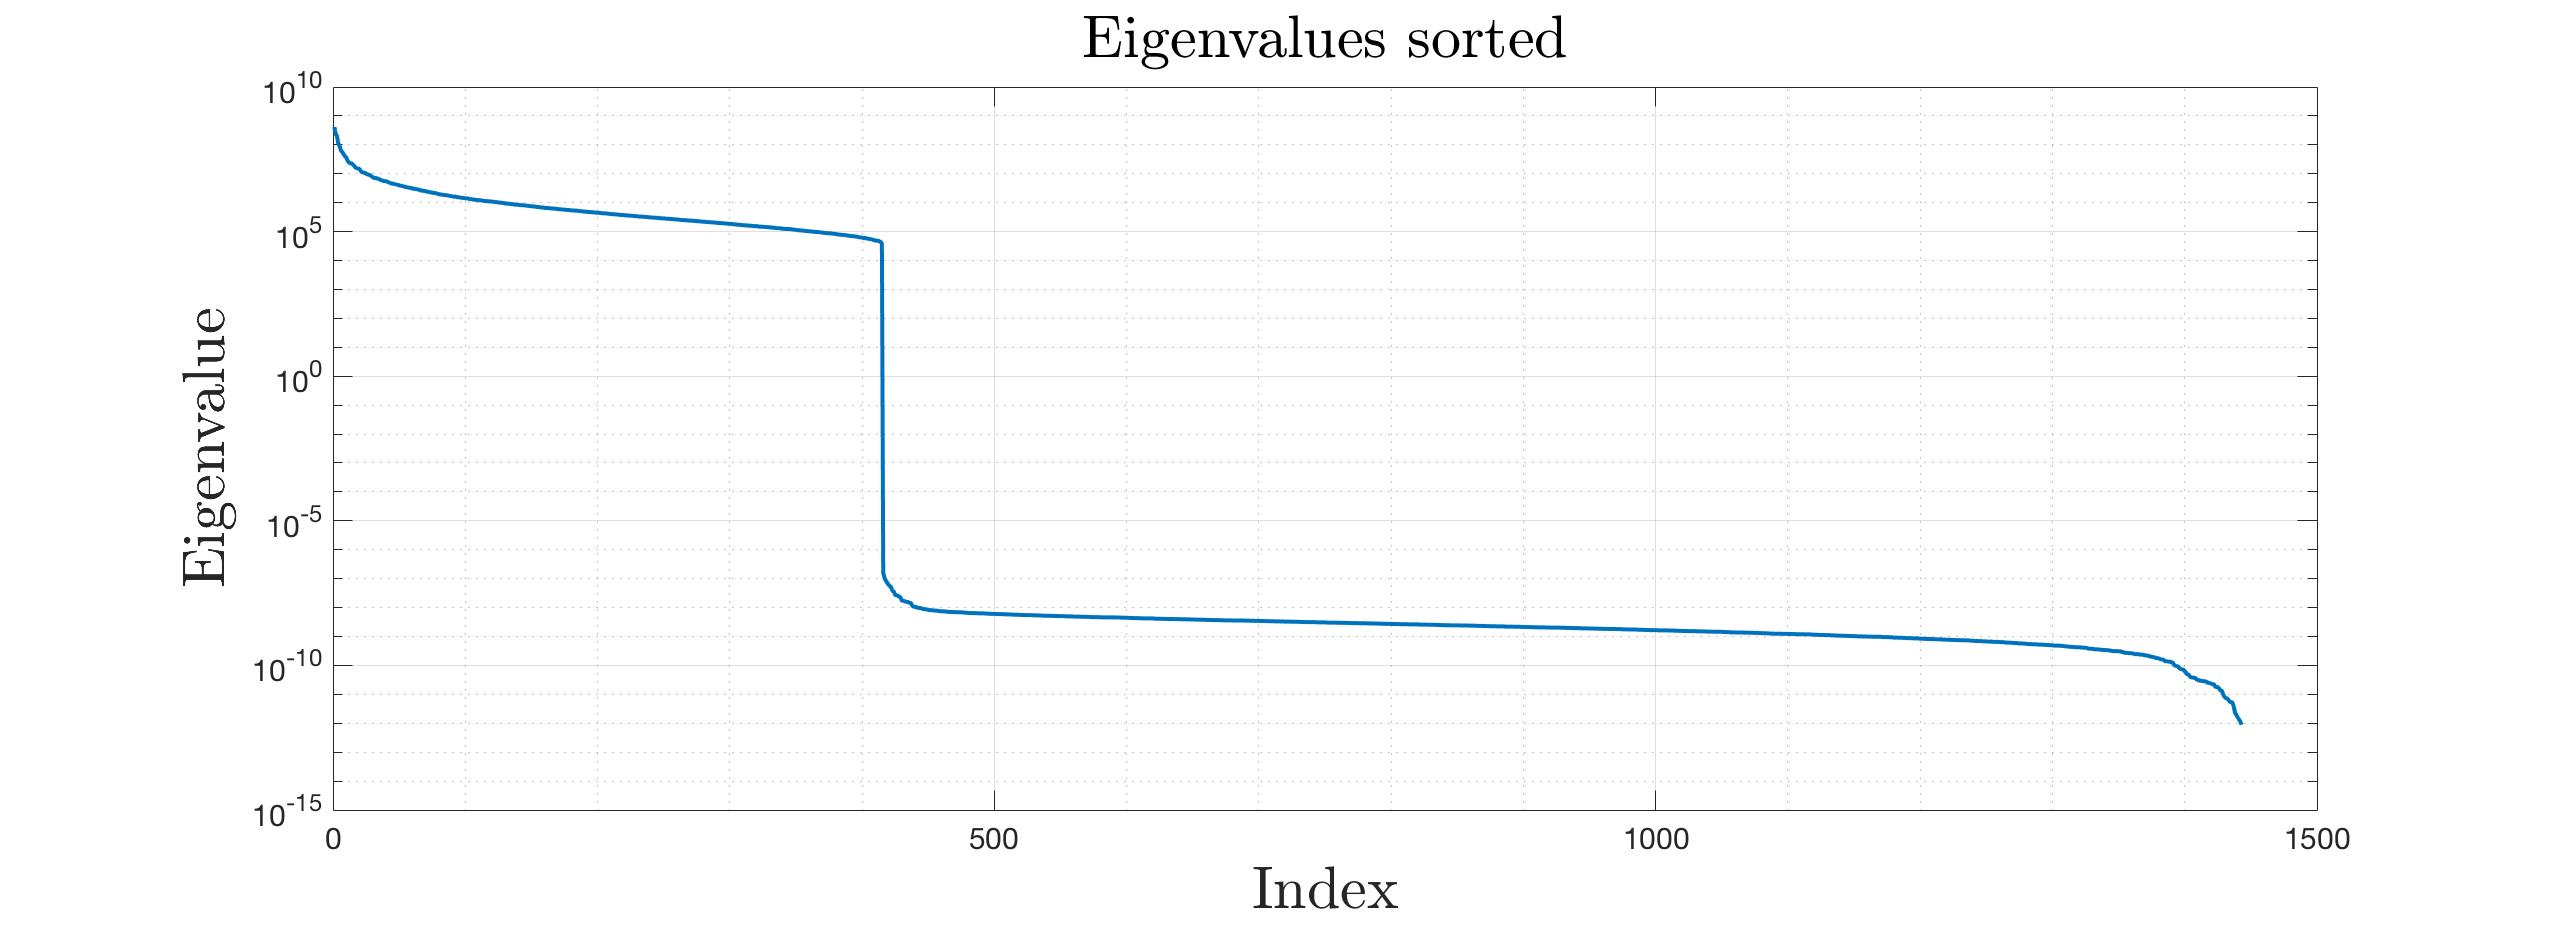
\includegraphics[width=0.5\textwidth]{../results/Q1A_PCA_Eigenvalues}

  \caption{Sorted Eigenvalues of Covariance Matrix $S$ \label{fig:Eig1}}

\end{figure}

It can be seen that first 415 values are much greater than 1. The \nth{416} value is around $10^{-10}$. The three best eigenvectors, or eigenfaces corresponding to the three highest eigenvalues are shown below in Figure \ref{fig:Eig2} . Finally the mean face which was initially subtracted from the face data is shown in Figure \ref{fig:Mean} .


\begin{figure}[H]

\centering
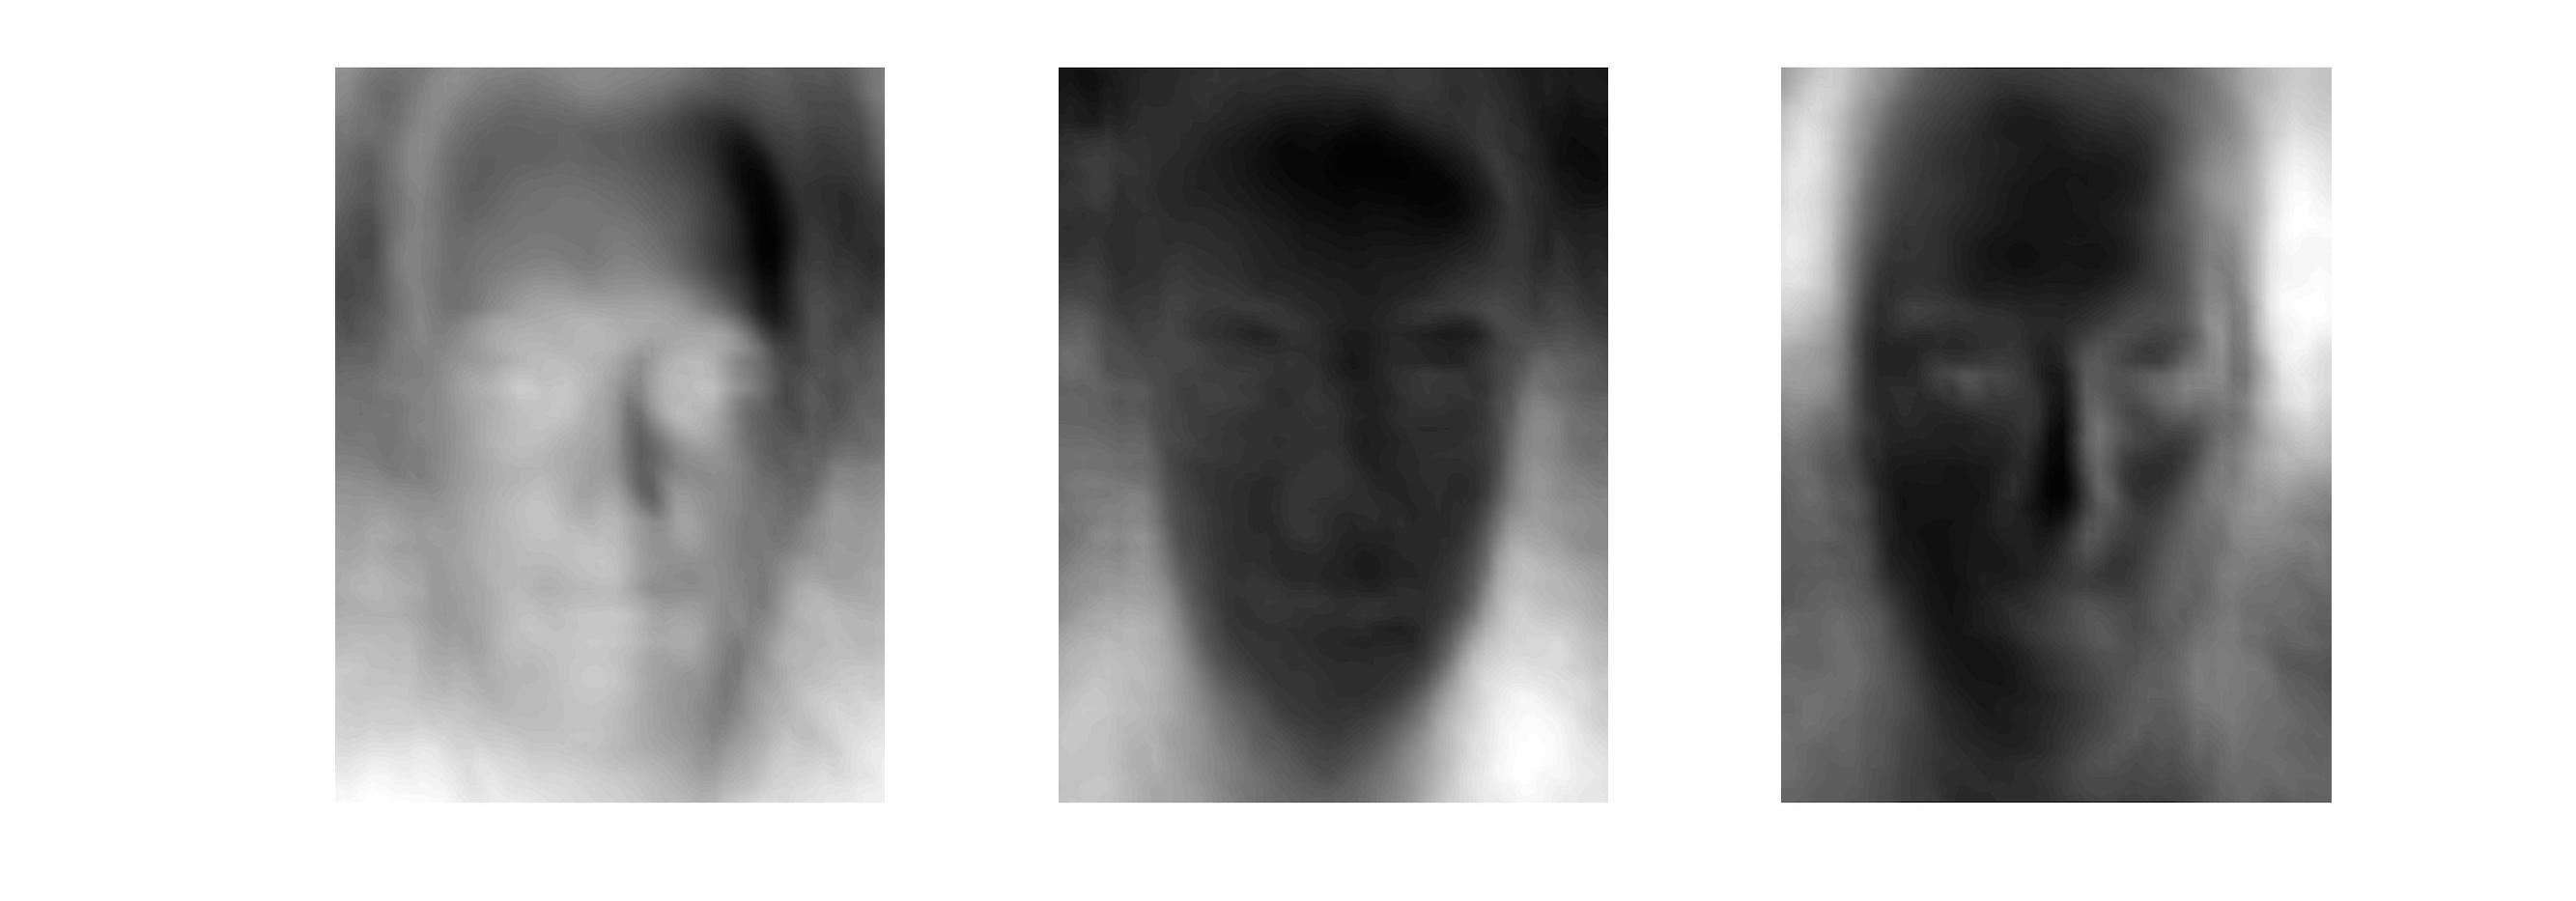
\includegraphics[width=0.5\textwidth]{../results/Q1A_PCA_Eigenfaces}

  \caption{Best 3 Eigenfaces of Covariance Matrix $S$ \label{fig:Eig2}}

\centering
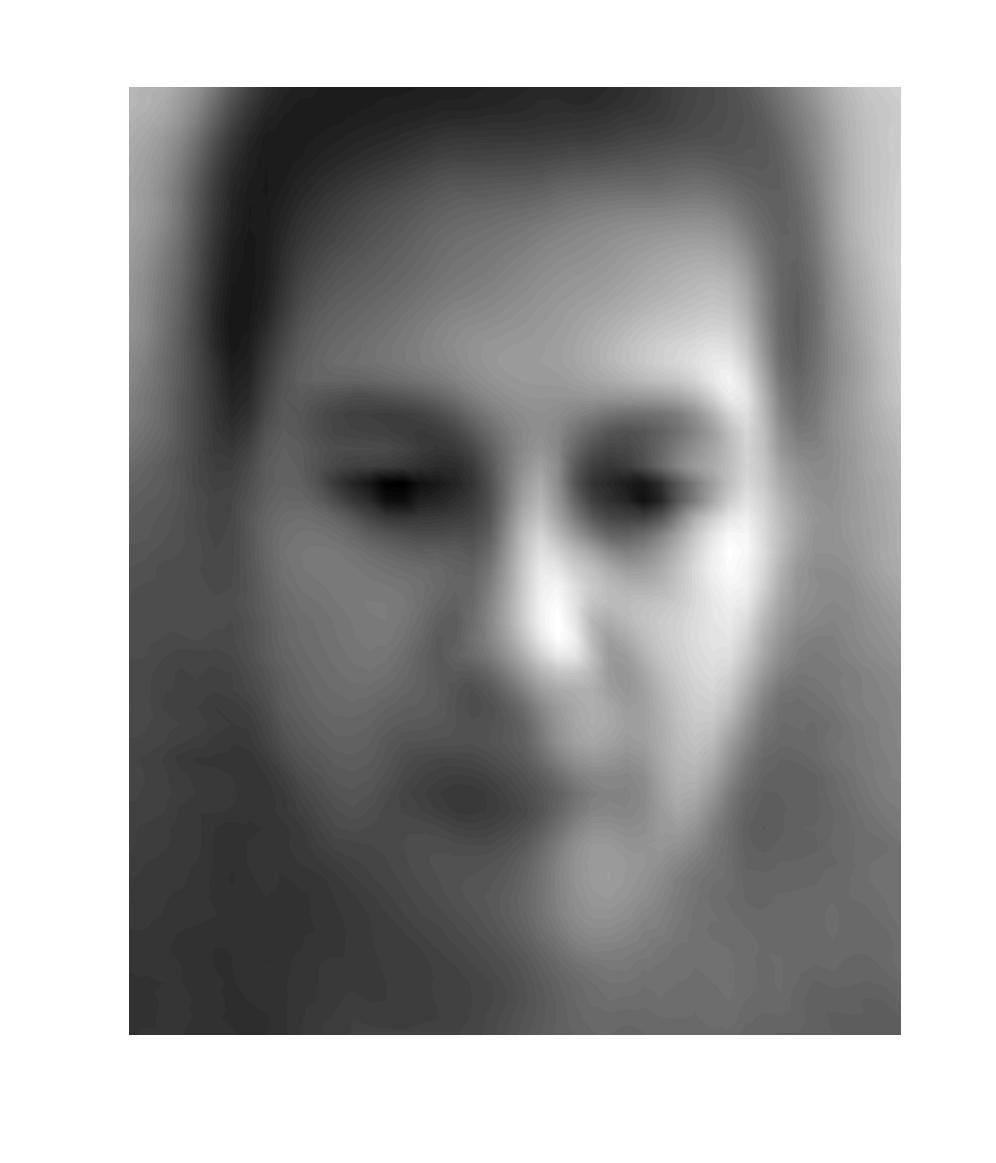
\includegraphics[width=0.15\textwidth]{../results/Q1A_PCA_Mean}

  \caption{Mean Face from {\tt\small training} \label{fig:Mean}}


\centering
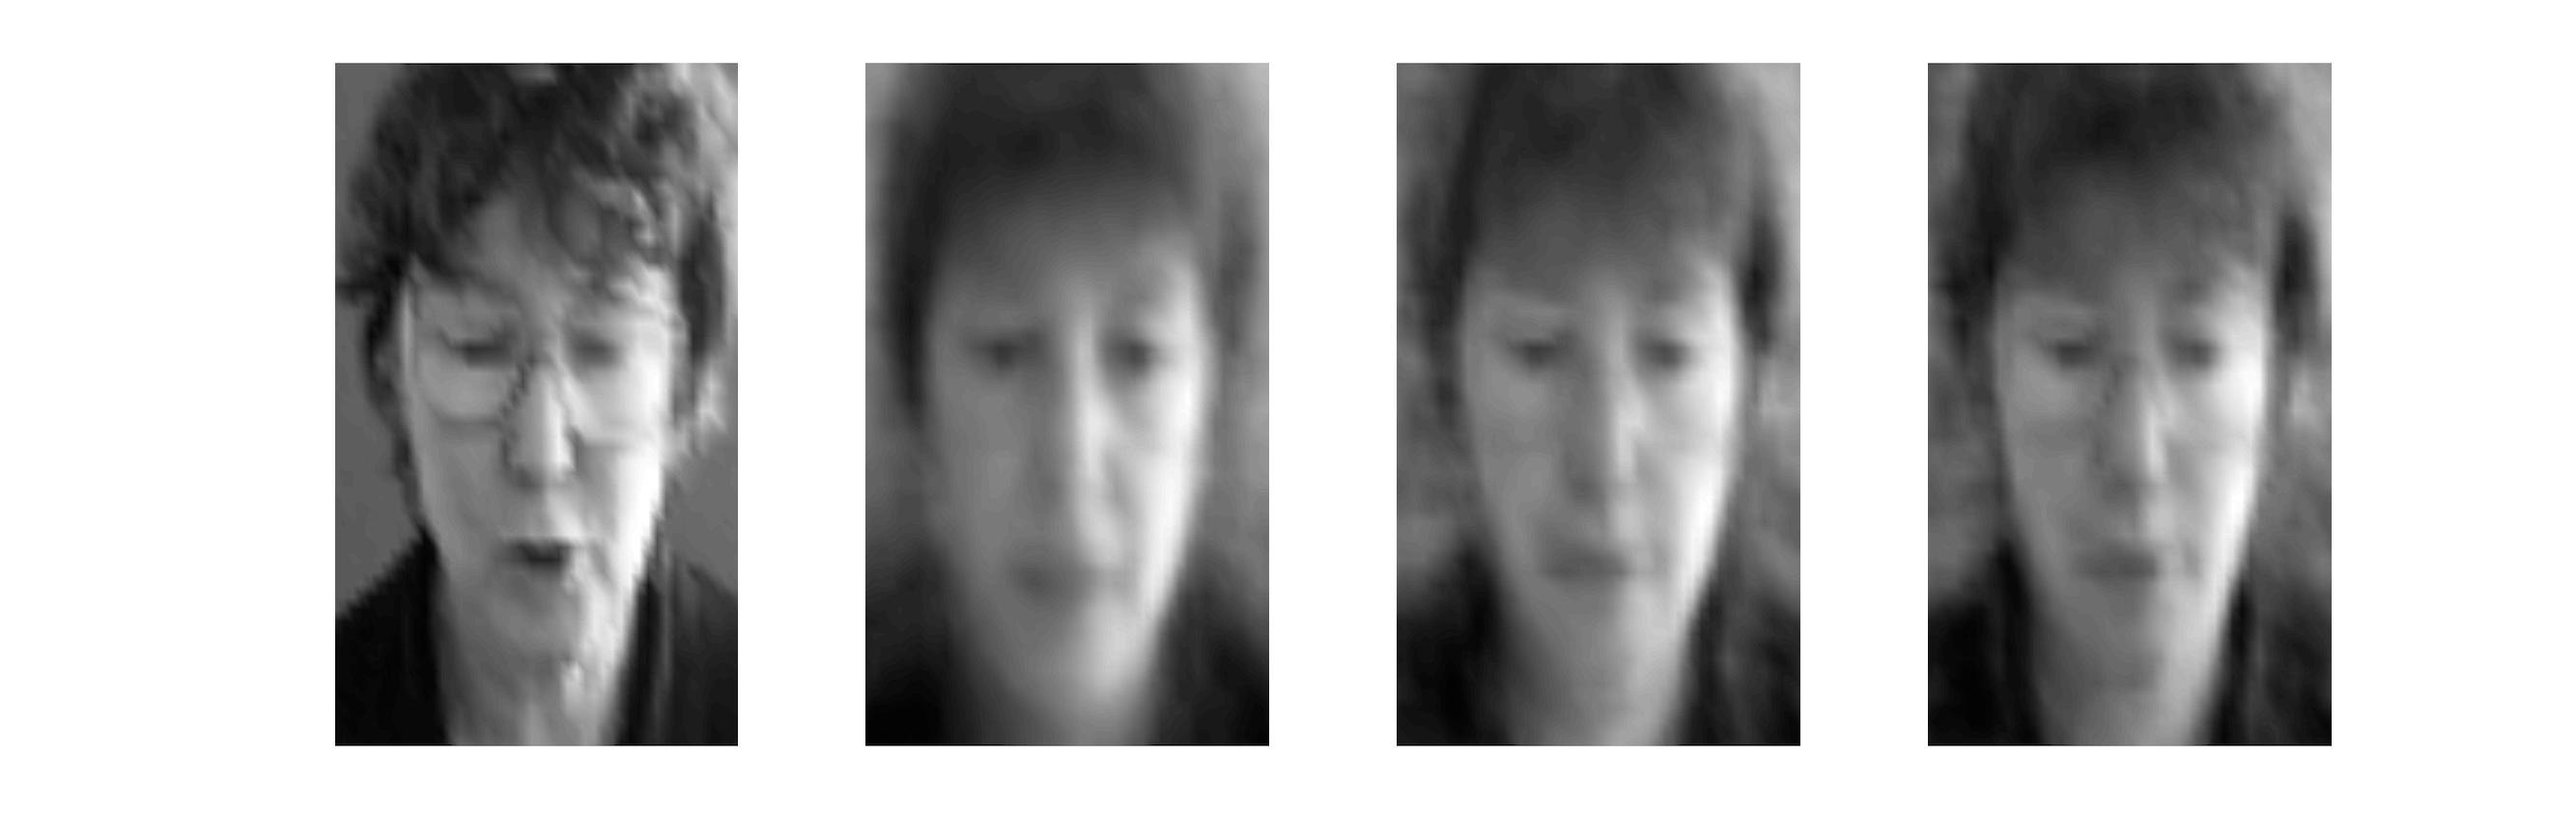
\includegraphics[width=0.5\textwidth]{../results/Q2A_PCA_Reco}

  \caption{Comparison of Reconstruted Images: Original Image, 20 Eigenfaces, 50 Eigenfaces, 80 Eigenfaces \label{fig:Reco}}

\end{figure}


We have determined empirically that using just 80 out of 415 eigenvectors is suitable for facial recognition - Figure \ref{fig:Reco}. This constitutes a compromise between accuracy and performance, by reducing the problem dimensionality.
\subsubsection{\boldmath$A^TA$}
Alternatively as suggested earlier we could compute a covariance matrix $S_T = \frac{1}{416} \times A^TA$, which now has dimensions of $416 \times 416$ instead of $2576 \times 2576$. We know \cite{Data Mining} that both matrices produce the same (meaningful) eigenvectors and eigenvalues. The plot of the latter in the  descending order shown in Figure \ref{fig:Eig3} proves the above claim.

\begin{figure}[H]
\centering
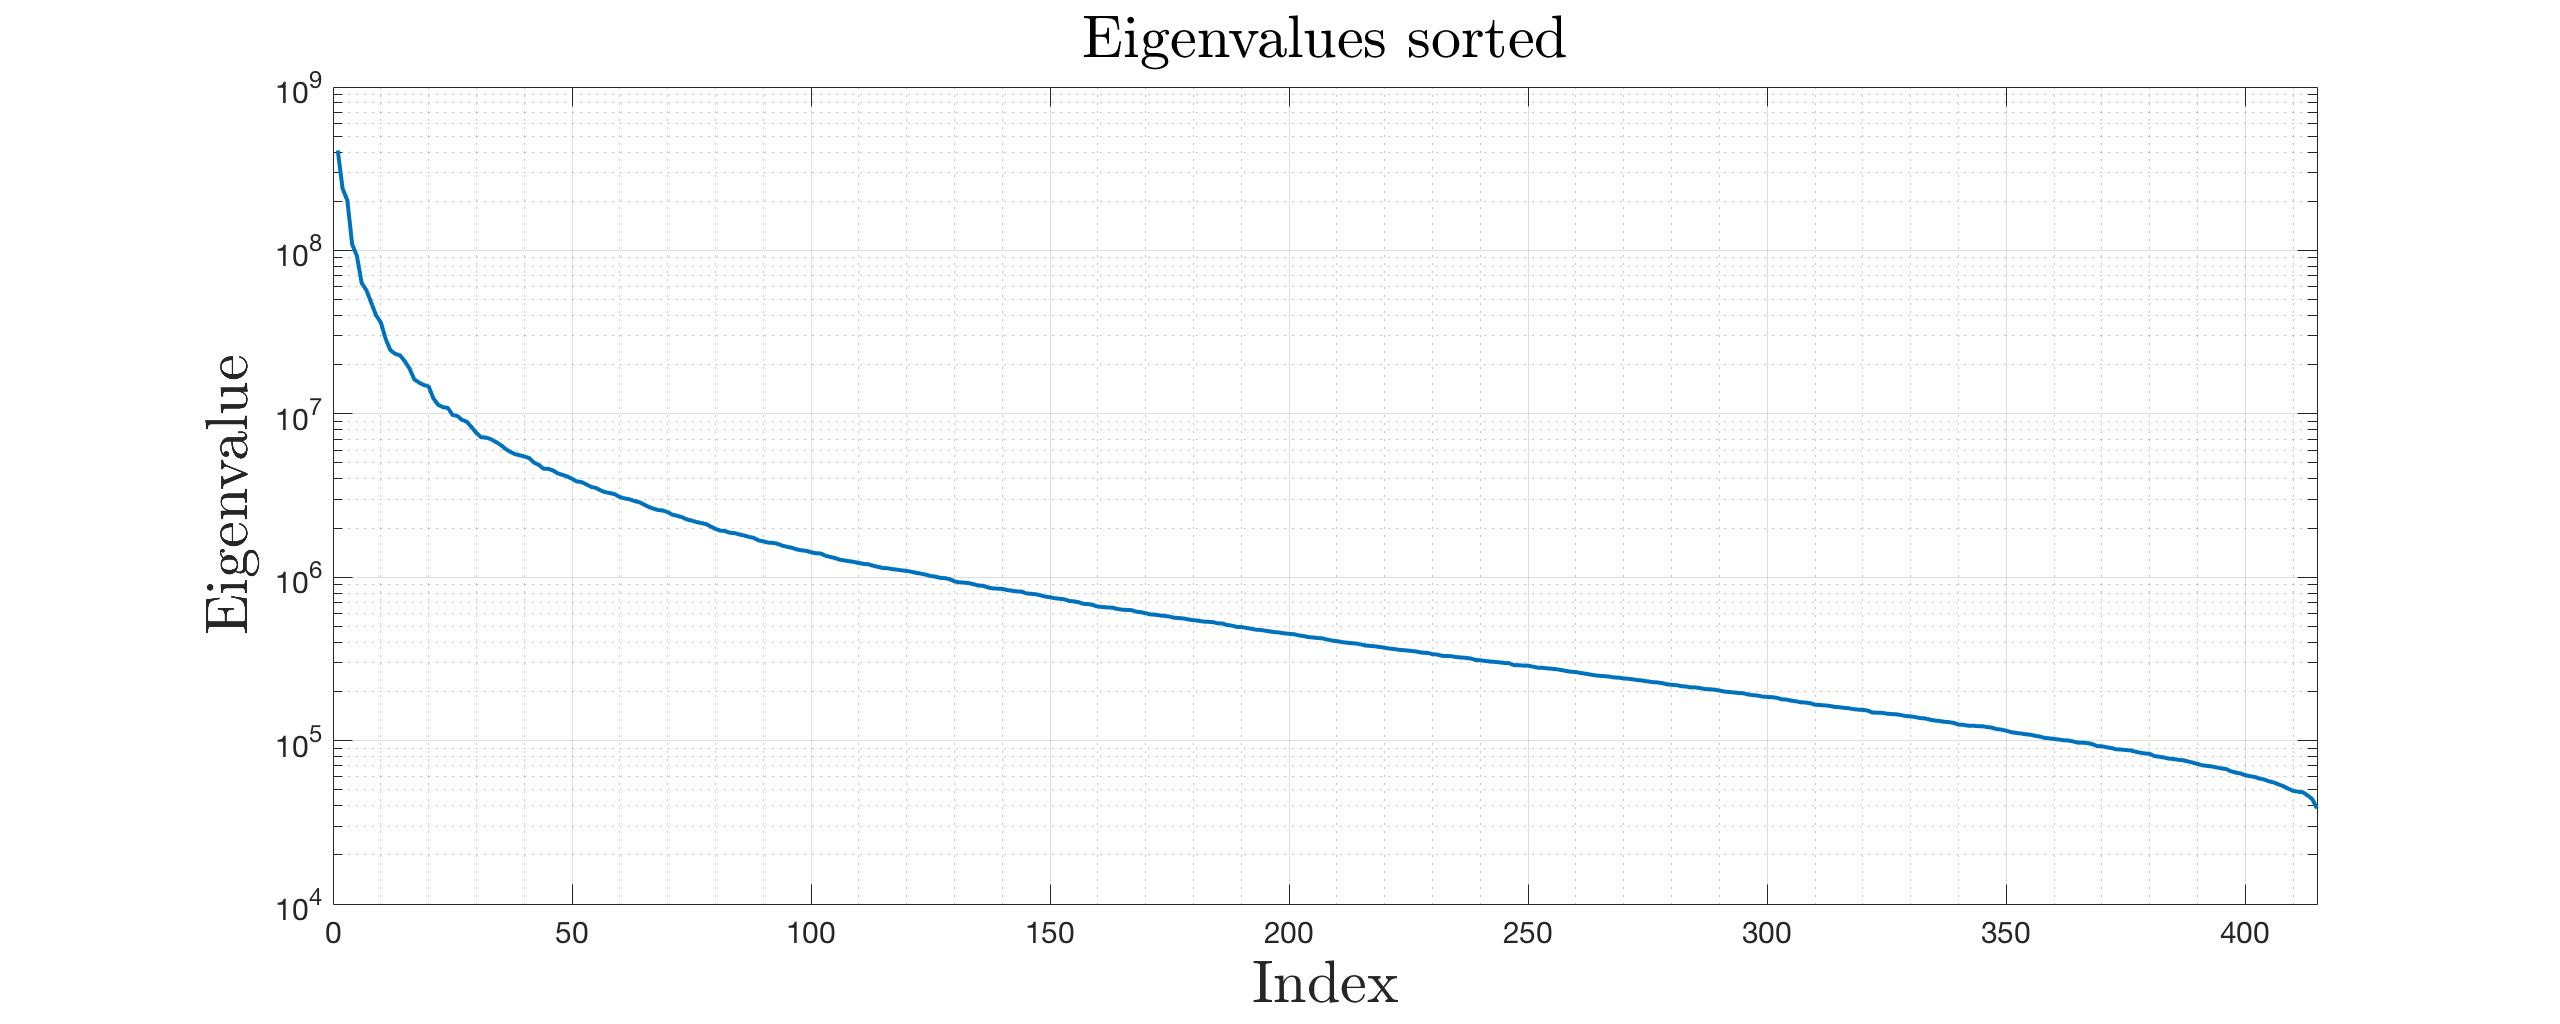
\includegraphics[width=0.5\textwidth]{../results/Q1B_PCA_Eigenvalues}

  \caption{Eignevalues of $S_T$ \label{fig:Eig3}}

\end{figure}

\subsection{DAYYYUUM}
\begin{quote}
\begin{center}
     An analysis of the frobnicatable foo filter.
\end{center}

   In this paper we present a performance analysis of the
   paper of Smith \etal [1], and show it to be inferior to
   all previously known methods.  Why the previous paper
   was accepted without this analysis is beyond me.

   [1] Smith, L and Jones, C. ``The frobnicatable foo
   filter, a fundamental contribution to human knowledge''.
   Nature 381(12), 1-213.
\end{quote}


\begin{quotation}
\noindent
   We describe a system for zero-g frobnication.  This
   system is new because it handles the following cases:
   A, B.  Previous systems [Zeus et al. 1968] didn't
   handle case B properly.  Ours handles it by including
   a foo term in the bar integral.

   ...

   The proposed system was integrated with the Apollo
   lunar lander, and went all the way to the moon, don't
   you know.  It displayed the following behaviours
   which show how well we solved cases A and B: ...
\end{quotation}



\section{Final copy}

You must include your signed IEEE copyright release form when you submit
your finished paper. We MUST have this form before your paper can be
published in the proceedings.


{\small
\bibliographystyle{ieee}
\bibliography{egbib}
}

\begin{thebibliography}{9}
\bibitem{Data Mining} 
Inderjit Dhillon. 
\textit{CS 391D Data Mining: A Mathematical Perspective Fall 2009}. 
The University of Texas at Austin, September 2009.
\end{thebibliography}
\end{document}
